\clearpage
\section{Matched Interventions and Complete Outcomes}

\subsection{Input geometry and what the cap bounds}
Write the native proposal for one output unit as $\bar u_j=[\Delta W_{j:},\Delta b_j]^\top\in\R^{d+1}$, and augment the current input matrix as $\bar H=[H,\mathbf1_n]$. The direct affine RMS satisfies
\begin{equation}
 s_j^2=\bar u_j^\top G\bar u_j,\qquad G=\bar H^\top\bar H/n.
\end{equation}
The input second moment is uncentered. A factor $\gamma_j=\min(1,\tau/s_j)$ radially rescales the entire proposal for one output unit, retaining its within-row direction while ensuring $\gamma_js_j\leq\tau$ for $\tau>0$, up to stored FP32 rounding. It neither computes the nearest Euclidean projection nor inverts $G$. A zero score leaves the proposal unchanged, and a calibrated zero threshold disables that site's cap.

For simultaneous upstream and local updates, actual preactivation change is
\begin{equation}
 \Delta Z=
 \underbrace{H(\Delta W^{\rm cap})^\top+\mathbf1_n(\Delta b^{\rm cap})^\top}_{\text{bounded direct term}}
 +\underbrace{\Delta H W^\top+\Delta H(\Delta W^{\rm cap})^\top}_{\text{unconstrained upstream and interaction terms}}.
\end{equation}
The local rule therefore does not bound total propagated representation movement, complete attention output, network output, or loss. Its distinction from relative representation-change correction, AGC, and neuron-space descent is described in the main related work~\cite{kosson2024warmup,brock2021normalization,benzing2022neurons}. Those methods are relevant comparators for a future superiority claim; the present four-family experiment does not implement them.

The controller captures current reference-set inputs once and evaluates local products with the native stored Adam increments. It does not need a separate altered-network forward for every candidate unit. Convolutional scores account for receptive-field patches, with the original stride, padding, and site structure; absent bias increments are zero. The two MLP hidden affines, 31 ResNet convolutions, and two QKV/four feed-forward Transformer affines are targeted. Output heads and all other untargeted parameters keep native increments. Moments and clocks advance normally, and the accepted parameters are checked against the actual stored-increment bounds.

\subsection{Matched design, calibration, and validation coverage}
All 12 conditions within a model share its complete pre-treatment model/optimizer/random state, data order, and numerical configuration. Treatment starts at $512\to513$, $256\to257$, or $544\to545$, and continues through completed states 800/576/928. The unchanged control is included in every comparison. The 36 conditions contain 11,904 total continuation updates, of which 10,912 are in treated arms. Baseline training rates are $.001/.003/.003$. Immediate rate multipliers are $.75/.5/.1$; late second-moment coefficients are $.95/.9/.5$; complete raw-gradient clipping thresholds are $.5/1$; and cap quantiles are q25/q50/q75. No ramp, moment reset, loss-triggered delay, or additional method is bundled into these interventions.

One scalar budget per target site is the linearly interpolated quantile of all its per-unit native scores pooled over the eight untreated outgoing states $t_0-8,\ldots,t_0-1$. The reference set and native rate are the same as in the unchanged continuation. Budgets are frozen before the first treated update and remain fixed as current inputs and moments evolve. q50 was selected before the matched outcomes. The main motion illustration now uses q25 after inspection of training outcomes; it is not presented as a prespecified selection or a universal optimum.

Qualification includes common eight-update fingerprints across workers, 108 exact audits of the full gradient, reference-example evaluation, and native proposal, calibration-pool reconstruction, stored-increment bounds, observer invariance, and terminal full-state evaluation. These verify the executed comparisons; they are not additional statistical replications. One initialization per model supplies no seed-level confidence interval, and different settings have unequal effective strengths.

All 10,000 CIFAR-10 test images and 245,550 WikiText-2 test tokens are evaluated at the five fixed states $t_0$, $t_0+32$, $(t_0+t_f)/2$, $t_f-32$, and $t_f$. Transformer validation also covers all 217,630 valid targets. These sparse trajectories cannot establish the timing or absence of held-out spikes. No evaluation state or setting is selected using held-out loss.

\subsection{Metrics, complete values, and costs}
Mean training loss excludes the shared start state, averaging $t_0+1,\ldots,t_f$. Positive variation sums $\max(L_t-L_{t-1},0)$ over those transitions. The last-32 mean uses $t_f-31,\ldots,t_f$. Final loss is $L_{t_f}$. Percentage loss changes are $100(x/x_{\rm Adam}-1)$; Positive-variation reduction is $100(1-\mathcal P/\mathcal P_{\rm Adam})$. Lowering $\mathcal P$ alone can reward slower progress, and a finite-window mean is not a convergence rate.

For site motion, both baseline and treatment RMS divide by the same unchanged-Adam maximum for that site over the complete post-treatment window. Cosine spans $[-1,1]$. Within each supplementary plate, the RMS color scale includes all observed values across the three cases; different plates may use different maxima. Dashed vertical lines mark the baseline's largest relative excursion peak, not a treatment trigger. The main q25 plate uses the same underlying q25 values with a compact layout, logarithmic losses, and no peak markers.

The following three tables retain absolute final/late losses alongside all relative effects. The main compact table reports absolute training outcomes; retained CSVs supply every scalar and validation outcome.
\begin{table}[H]
\centering
\small
\setlength{\tabcolsep}{4pt}
\begin{tabular}{lrrrrr}
\toprule
Setting & \shortstack{PV reduction\\(\%)} & \shortstack{Mean loss\\change (\%)} & \shortstack{Final\\loss} & \shortstack{Last-32\\loss} & \shortstack{Test loss\\change (\%)} \\
\midrule
Unchanged Adam & 0 & 0 & 0.03025 & 0.01346 & 0 \\
LR $\times0.75$ & 17.51 & -16.65 & 0.01231 & 0.01601 & -2.307 \\
LR $\times0.5$ & 99 & -25.04 & 0.01073 & 0.01115 & -2.543 \\
LR $\times0.1$ & 99.58 & -3.336 & 0.01849 & 0.01866 & -8.509 \\
$\beta_2=0.95$ & -125 & 16.78 & 0.01917 & 0.01795 & -2.922 \\
$\beta_2=0.9$ & -77.96 & 18.16 & 0.01588 & 0.01931 & -3.876 \\
$\beta_2=0.5$ & -187.5 & 127 & 0.03476 & 0.03551 & -11.06 \\
Clip 0.5 & -65.32 & 2.084 & 0.01669 & 0.01675 & -3.119 \\
Clip 1.0 & -419.3 & 48.01 & 0.02442 & 0.06413 & -7.75 \\
Cap q25 & 75.32 & -30.87 & 0.009722 & 0.009742 & -0.1062 \\
Cap q50 & 87.75 & -32.18 & 0.008691 & 0.009076 & 0.5332 \\
Cap q75 & 97.46 & -27.86 & 0.0105 & 0.01067 & 0.02148 \\
\bottomrule
\end{tabular}
\caption{CIFAR-10 / MLP. Matched initialization-0 interventions at states 512--800. PV is positive loss variation. Mean excludes the common fork; late loss averages the final 32 states. Test changes use the complete held-out split. All changes compare with unchanged Adam; no held-out selection.}
\end{table}

\begin{table}[H]
\centering
\small
\setlength{\tabcolsep}{4pt}
\begin{tabular}{lrrrrr}
\toprule
Setting & \shortstack{PV reduction\\(\%)} & \shortstack{Mean loss\\change (\%)} & \shortstack{Final\\loss} & \shortstack{Last-32\\loss} & \shortstack{Test loss\\change (\%)} \\
\midrule
Unchanged Adam & 0 & 0 & 0.006702 & 0.008241 & 0 \\
LR $\times0.75$ & -26.45 & 16.81 & 0.02184 & 0.02845 & -11.37 \\
LR $\times0.5$ & -11.11 & 27.2 & 0.05446 & 0.07608 & -22.67 \\
LR $\times0.1$ & 98.98 & 89.46 & 0.2447 & 0.2542 & -45.55 \\
$\beta_2=0.95$ & -250.3 & 28.46 & 0.1142 & 0.3079 & -32.14 \\
$\beta_2=0.9$ & -63.32 & -3.529 & 0.02139 & 0.08911 & 2.459 \\
$\beta_2=0.5$ & 21.75 & 6.279 & 0.05511 & 0.04997 & 11.85 \\
Clip 0.5 & -2.559 & 14.52 & 0.05778 & 0.07538 & -19.91 \\
Clip 1.0 & -85.65 & 13.27 & 0.06199 & 0.07824 & -15.01 \\
Cap q25 & 36.09 & -21.56 & 0.00493 & 0.005935 & 9.557 \\
Cap q50 & 2.771 & -9.424 & 0.008044 & 0.01001 & 2.424 \\
Cap q75 & 66.14 & -19.48 & 0.004833 & 0.005969 & 10.8 \\
\bottomrule
\end{tabular}
\caption{CIFAR-10 / ResNet-32. Matched initialization-0 interventions at states 256--576. PV is positive loss variation. Mean excludes the common fork; late loss averages the final 32 states. Test changes use the complete held-out split. All changes compare with unchanged Adam; no held-out selection.}
\end{table}

\begin{table}[H]
\centering
\small
\setlength{\tabcolsep}{4pt}
\begin{tabular}{lrrrrr}
\toprule
Setting & \shortstack{PV reduction\\(\%)} & \shortstack{Mean loss\\change (\%)} & \shortstack{Final\\loss} & \shortstack{Last-32\\loss} & \shortstack{Test loss\\change (\%)} \\
\midrule
Unchanged Adam & 0 & 0 & 0.9178 & 0.9937 & 0 \\
LR $\times0.75$ & 37.9 & -2.982 & 0.614 & 0.6306 & 8.338 \\
LR $\times0.5$ & 66 & -11.36 & 0.6277 & 0.6483 & 8.675 \\
LR $\times0.1$ & 100 & -5.522 & 0.7572 & 0.7606 & -7.273 \\
$\beta_2=0.95$ & -7.139 & -10.67 & 0.593 & 0.7318 & 29.25 \\
$\beta_2=0.9$ & 29.71 & -16.84 & 0.6067 & 0.6055 & 40.2 \\
$\beta_2=0.5$ & 79.61 & -9.626 & 0.6462 & 0.6529 & 34.8 \\
Clip 0.5 & 87.71 & -17.79 & 0.617 & 0.6162 & 18.32 \\
Clip 1.0 & 65.56 & -15.58 & 0.6201 & 0.6251 & 21.74 \\
Cap q25 & 89.16 & -18.47 & 0.5505 & 0.5825 & 26.55 \\
Cap q50 & 96.23 & -19.84 & 0.7039 & 0.6065 & 27.52 \\
Cap q75 & 98.77 & -19.78 & 0.5833 & 0.5866 & 28.7 \\
\bottomrule
\end{tabular}
\caption{WikiText-2 / Transformer. Matched initialization-0 interventions at states 544--928. PV is positive loss variation. Mean excludes the common fork; late loss averages the final 32 states. Test changes use the complete held-out split. All changes compare with unchanged Adam; no held-out selection.}
\end{table}

\clearpage
\begin{table}[H]
\centering\small
\setlength{\tabcolsep}{4pt}
\begin{tabular}{llrrrrr}
\toprule
Case & Setting & \shortstack{Gradient\\ms/boundary} & \shortstack{Probe capture\\ms/boundary} & \shortstack{Adam\\ms/update} & \shortstack{Controller\\ms/update} & \shortstack{Peak\\GiB} \\
\midrule
MLP & Adam & 6.181 & 2.088 & 0.2696 & 0.003871 & 0.422 \\
MLP & Cap q50 & 4.418 & 3.247 & 0.2733 & 41.76 & 0.616 \\
ResNet-32 & Adam & 3402 & 17.58 & 3.172 & 0.006511 & 4.35 \\
ResNet-32 & Cap q50 & 3462 & 24.12 & 8.536 & 292 & 4.35 \\
Transformer & Adam & 8312 & 8.875 & 2.287 & 0.01303 & 4.65 \\
Transformer & Cap q50 & 9516 & 10.17 & 2.555 & 12.57 & 4.66 \\
\bottomrule
\end{tabular}
\caption{Synchronized components on the recorded GPU class: GB10 for MLP, RTX4090 for ResNet-32 and RTX5090 for Transformer. Gradient/probe means include every boundary, including the terminal state; Adam/controller means cover updates only. Probe time covers forward capture and cap inputs. Cosine/RMS reductions, other scalar diagnostics, logging and checkpoint I/O lie in the separately retained remaining wall time. Controller time alone is not deployable overhead. Peak is the process high-water allocation through the arm, not an isolated per-method peak. Hosts may differ within a GPU class; no cross-host speed ranking is implied. Full-grid timings are retained separately.}
\end{table}


Component times are synchronized on the stated GPU classes, but hosts and instrumentation differ. Gradient and reference-evaluation means include the terminal boundary; optimizer/controller means count updates only. Extra diagnostics, reductions, logging, and I/O occupy remaining wall time. Memory is a process high-water allocation through an arm. In particular, the MLP q50 controller's 41.8 ms/update versus 4.4 ms/full-gradient boundary rules out describing this implementation as negligible-cost. These measurements do not establish a clean time-to-loss comparison.

\clearpage
\clearpage
\begin{figure}[H]
\centering
\includegraphics[page=1,width=7.15in]{\vcassetroot/figures/17-matched-intervention-loss.pdf}
\caption{Complete loss trajectories for all four intervention families. Each column repeats the same unchanged-Adam control and logarithmic scale. Every state in the fixed 512--800, 256--576, and 544--928 windows is retained, without smoothing. Only the family named by each row changes; one initialization per model.}
\end{figure}
\clearpage
\begin{figure}[H]
\centering
\includegraphics[page=1,width=7.15in]{\vcassetroot/figures/21-matched-heldout-loss.pdf}
\caption{Complete test loss at the five fixed evaluation states. Each CIFAR-10 evaluation uses all 10,000 test images; Transformer evaluations use all 245,550 valid test tokens. Lines join only measured states. These observations are not used for checkpoint or setting selection, and cannot resolve intervening held-out excursions.}
\end{figure}
\clearpage
\begin{figure}[H]
\centering
\includegraphics[page=1,width=7.15in]{\vcassetroot/figures/22-matched-update-and-controller-activity.pdf}
\caption{Actual stored parameter-increment norms for every treatment and unchanged Adam. Logarithmic scales are shared within each model. Equal nominal coefficients do not imply matched applied parameter or functional movement; these curves retain their resulting differences.}
\end{figure}
\clearpage
\begin{figure}[H]
\centering
\includegraphics[page=2,width=7.15in]{\vcassetroot/figures/22-matched-update-and-controller-activity.pdf}
\caption{Controller activity: retained raw-gradient factors for global clipping and fractions of targeted units capped for q25/q50/q75. Clipping changes the optimizer input; the cap changes native stored increments while retaining advanced moments. Values are placed at completed-update endpoints.}
\end{figure}
\clearpage
\begin{figure}[H]
\centering
\includegraphics[page=1,width=7.15in]{\vcassetroot/figures/20-matched-all-setting-stage-heatmaps.pdf}
\caption{LR $\times.75$ versus unchanged Adam over the complete matched windows. Rows retain full loss, baseline/treatment change cosine, and baseline/treatment RMS. Each stage uses the same baseline RMS denominator for both arms. Color limits include every value and may differ across plates. Dashed lines are descriptive baseline peak references.}
\end{figure}
\clearpage
\begin{figure}[H]
\centering
\includegraphics[page=2,width=7.15in]{\vcassetroot/figures/20-matched-all-setting-stage-heatmaps.pdf}
\caption{LR $\times.5$ versus unchanged Adam over the complete matched windows. Rows retain full loss, baseline/treatment change cosine, and baseline/treatment RMS. Each stage uses the same baseline RMS denominator for both arms. Color limits include every value and may differ across plates. Dashed lines are descriptive baseline peak references.}
\end{figure}
\clearpage
\begin{figure}[H]
\centering
\includegraphics[page=3,width=7.15in]{\vcassetroot/figures/20-matched-all-setting-stage-heatmaps.pdf}
\caption{LR $\times.1$ versus unchanged Adam over the complete matched windows. Rows retain full loss, baseline/treatment change cosine, and baseline/treatment RMS. Each stage uses the same baseline RMS denominator for both arms. Color limits include every value and may differ across plates. Dashed lines are descriptive baseline peak references.}
\end{figure}
\clearpage
\begin{figure}[H]
\centering
\includegraphics[page=4,width=7.15in]{\vcassetroot/figures/20-matched-all-setting-stage-heatmaps.pdf}
\caption{$\beta_2=.95$ versus unchanged Adam over the complete matched windows. Rows retain full loss, baseline/treatment change cosine, and baseline/treatment RMS. Each stage uses the same baseline RMS denominator for both arms. Color limits include every value and may differ across plates. Dashed lines are descriptive baseline peak references.}
\end{figure}
\clearpage
\begin{figure}[H]
\centering
\includegraphics[page=5,width=7.15in]{\vcassetroot/figures/20-matched-all-setting-stage-heatmaps.pdf}
\caption{$\beta_2=.9$ versus unchanged Adam over the complete matched windows. Rows retain full loss, baseline/treatment change cosine, and baseline/treatment RMS. Each stage uses the same baseline RMS denominator for both arms. Color limits include every value and may differ across plates. Dashed lines are descriptive baseline peak references.}
\end{figure}
\clearpage
\begin{figure}[H]
\centering
\includegraphics[page=6,width=7.15in]{\vcassetroot/figures/20-matched-all-setting-stage-heatmaps.pdf}
\caption{$\beta_2=.5$ versus unchanged Adam over the complete matched windows. Rows retain full loss, baseline/treatment change cosine, and baseline/treatment RMS. Each stage uses the same baseline RMS denominator for both arms. Color limits include every value and may differ across plates. Dashed lines are descriptive baseline peak references.}
\end{figure}
\clearpage
\begin{figure}[H]
\centering
\includegraphics[page=7,width=7.15in]{\vcassetroot/figures/20-matched-all-setting-stage-heatmaps.pdf}
\caption{Clipping .5 versus unchanged Adam over the complete matched windows. Rows retain full loss, baseline/treatment change cosine, and baseline/treatment RMS. Each stage uses the same baseline RMS denominator for both arms. Color limits include every value and may differ across plates. Dashed lines are descriptive baseline peak references.}
\end{figure}
\clearpage
\begin{figure}[H]
\centering
\includegraphics[page=8,width=7.15in]{\vcassetroot/figures/20-matched-all-setting-stage-heatmaps.pdf}
\caption{Clipping 1 versus unchanged Adam over the complete matched windows. Rows retain full loss, baseline/treatment change cosine, and baseline/treatment RMS. Each stage uses the same baseline RMS denominator for both arms. Color limits include every value and may differ across plates. Dashed lines are descriptive baseline peak references.}
\end{figure}
\clearpage
\begin{figure}[H]
\centering
\includegraphics[page=9,width=7.15in]{\vcassetroot/figures/20-matched-all-setting-stage-heatmaps.pdf}
\caption{Cap q25 versus unchanged Adam over the complete matched windows. Rows retain full loss, baseline/treatment change cosine, and baseline/treatment RMS. Each stage uses the same baseline RMS denominator for both arms. Color limits include every value and may differ across plates. Dashed lines are descriptive baseline peak references.}
\end{figure}
\clearpage
\begin{figure}[H]
\centering
\includegraphics[page=10,width=7.15in]{\vcassetroot/figures/20-matched-all-setting-stage-heatmaps.pdf}
\caption{Cap q50 versus unchanged Adam over the complete matched windows. Rows retain full loss, baseline/treatment change cosine, and baseline/treatment RMS. Each stage uses the same baseline RMS denominator for both arms. Color limits include every value and may differ across plates. Dashed lines are descriptive baseline peak references.}
\end{figure}
\clearpage
\begin{figure}[H]
\centering
\includegraphics[page=11,width=7.15in]{\vcassetroot/figures/20-matched-all-setting-stage-heatmaps.pdf}
\caption{Cap q75 versus unchanged Adam over the complete matched windows. Rows retain full loss, baseline/treatment change cosine, and baseline/treatment RMS. Each stage uses the same baseline RMS denominator for both arms. Color limits include every value and may differ across plates. Dashed lines are descriptive baseline peak references.}
\end{figure}


\clearpage
\subsection{Output movement and the traced ResNet event}
For the main q25 illustration, maximum output RMS jumps decrease by
92.7\%/33.0\%/45.1\% in MLP/ResNet/Transformer. Total squared output movement
changes by $-97.6\%/-2.5\%/-59.7\%$. Negative output-change cosine occurs in
49.7\%/59.7\%/88.5\% of updates. In the squared-loss MLP, 139 of 140 q25
loss rises above $10^{-8}$ have a negative linear term outweighed by the
positive quadratic term; the remaining rise also has a positive linear
term. The exact output-loss identity is verified for every recorded step.

For q50, the maximum output RMS jump decreases by 83.2\%/23.1\%/62.9\% in MLP/ResNet/Transformer. The proportion of output changes with negative cosine is 89.2\%/66.9\%/95.8\%, compared with 99.3\%/36.9\%/36.7\% under unchanged Adam. Total squared output movement changes by $-88.6\%/+39.7\%/-55.4\%$. Thus a lower maximum jump need not mean less cumulative movement or fewer reversals.

In ResNet's previously selected steps 390--450, q50 reduces maximum loss from $.4407$ to $.1736$ (60.6\%). Positive variation over the complete 256--576 continuation falls only 2.8\%, because later oscillations remain. The whole window is the primary intervention comparison. For the squared-loss MLP, all 161 unchanged-Adam and 70 q50 rises above $10^{-8}$ have a negative output-space linear term outweighed by the positive squared-movement term. These counts use actual output changes on all 5,000 training examples.

\subsection{Historical MLP replication and the larger-rate ablation}
Earlier MLP experiments support method sensitivity and replication, but use a different window and are not pooled into the main matched grid. The historical q50 distributed-cap comparison includes initializations 0/1/2. A separate complete MLP factorial experiment uses five cap quantiles (q25/q50/q75/q90/q99), three native rates ($.001/.002/.004$), and an uncapped control at each rate: 54 continuations over three initializations. Each starts from the untreated state 448 and includes 705 loss states through 1152. Budgets use the preceding eight native-rate updates and are held identical across rates within an initialization.

The cap reduces disruption from a larger nominal rate, but the across-initialization mean loss at each quantile is higher at $2\times/4\times$ than at $1\times$. At q50 and $1\times$, mean training loss is $.01333\pm.00095$ versus $.01774\pm.00036$ for original Adam (mean $\pm$ sample SD over three initializations). The paired mean reduction is 24.79\%, while the final-four test mean increases 3.37\%. This is supporting evidence with its own endpoints, not three-initialization confirmation of the new common-fork four-family ranking. The cross-model quantile-by-rate-by-initialization grid remains unexecuted.

\begin{figure}[H]
\centering
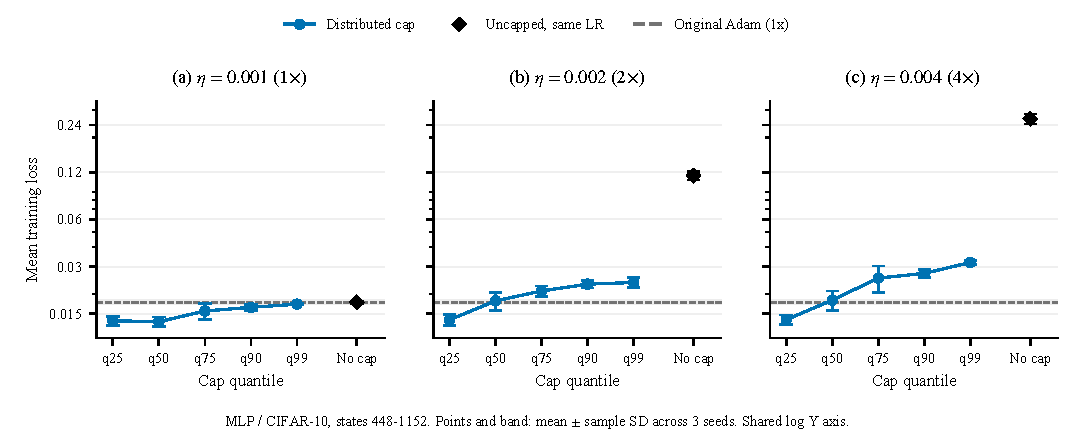
\includegraphics[width=7.15in]{figures/14-distributed-cap-quantile-ablation-mlp.pdf}
\caption{Historical MLP quantile-by-rate ablation across three initializations, with each treated branch compared with its same-rate unchanged-Adam control and with original Adam. Budgets are calibrated at the original rate and fixed across multipliers. The historical 448--1152 window differs from the main 512--800 MLP comparison. Increasing nominal rate does not improve mean training loss over the same cap at the original rate. The plotted uncertainty is sample variation across three initializations, not update-level replication.}
\end{figure}
